\documentclass[11pt]{article}
\usepackage[top=1.00in, bottom=1.0in, left=1.1in, right=1.1in]{geometry}
\renewcommand{\baselinestretch}{1.1}
\usepackage{graphicx}
\usepackage{natbib}
\usepackage{gensymb}
\usepackage{amsmath}
\usepackage{lineno}
\usepackage{xr-hyper}
\usepackage{longtable}
% \usepackage{tabularx}
% \usepackage{array}

\externaldocument{limitingcues}

\def\labelitemi{--}
\parindent=0pt

\usepackage{Sweave}
\begin{document}
\renewcommand{\thetable}{S\arabic{table}}
\renewcommand{\thefigure}{S\arabic{figure}}

\bibliographystyle{/Users/Lizzie/Documents/EndnoteRelated/Bibtex/styles/besjournals}
\renewcommand{\refname}{\CHead{}}
\begin{flushright}
Version dated: \today
\end{flushright}
\bigskip
\medskip
\begin{center}

\noindent{\Large {\bf Integrating experiments to predict interactive cue effects on spring phenology with warming}}\\ 
\bigskip

\noindent {\normalsize \sc
E. M. Wolkovich$^{1,2}$, C. J. Chamberlain$^{1,2}$, D. M. Buonaiuto$^{1,2}$, A. K. Ettinger$^{3}$ \\ \& I. Morales-Castilla$^{5}$}\\ % The lab in 2017 -- Lizzie, Ailene, Cat, Dan, Nacho

\noindent {\small \it
$^1$ Forest \& Conservation Sciences, Faculty of Forestry, University of British Columbia, 2424 Main Mall, Vancouver, BC V6T 1Z4\\
$^2$ Arnold Arboretum of Harvard University, 1300 Centre Street, Boston, Massachusetts, 02131, USA\\
$^3$ Organismic \& Evolutionary Biology, Harvard University, 26 Oxford Street, Cambridge, Massachusetts, 02138, USA\\
$^4$ The Nature Conservancy, 74 Wall Street, Seattle, Washington USA\\
$^5$ Global Change Ecology and Evolution Group, Department of Life Sciences, University of Alcal\`a, Alcal\`a de Henares 28805, Spain}
\end{center}



\section{Overview of OSPREE database}
% We could add info on ..
% types of events?
We built the Observed Spring Phenology Responses in Experimental Environments (OSPREE) database, by searching both ISI Web of Science and Google Scholar  the following terms: 
\begin{enumerate}
\item TOPIC = (budburst OR leaf-out) AND (photoperiod or daylength) AND temperature*, which yielded 85 publications
\item TOPIC = (budburst OR leaf-out) AND dorman*, which yielded 193 publications
\end{enumerate}
We extracted data (using ImageJ for figures, transcribing values from tables and extracting date, location and other methods from the text) from papers on woody plants that test for photoperiod and/or temperature effects on budburst, leafout, or flowering  (Fig. \ref{fig:datamap}). \citet{ettinger2020} used a subset of these data (studies on budburst for which we could estimate forcing, chilling and photoperiod treatments), while here we present the full database, capturing data from 84 papers (see Table \ref{tab:ref} for a list), of which 21 are focused on crops (\emph{Actinidia deliciosa, Malus domestica, Vitis vinifera, Ribes nigrum, Vaccinium ashei, Vaccinium corymbosum, Prunus persica}). Papers often reported more than one experiment, which we refer to as a `study.' \\

OSPREE includes 136 studies \citep[with the earliest study was conducted in 1947,see][]{Lamb:1948aa}, which spanned a variety of plant materials, though studies on `seedlings' (51 studies) and `cuttings' (55 studies) were most common. The most reported events were related to vegetative phases (days until or percent budburst or leafout, 66\% of events across studies), followed by flowering (12\% of events across studies). This is unsurprising given that species often leafout before flowering and most species' cuttings become resource limited after leafout and fail to reach flowering or later phenological stages.\\

\section{The chilling enigma of over-winter temperatures}
Our poor understanding of chilling makes estimating historical and predicted shifts in chilling difficult \citep{chuine2016}. Research to date suggests chilling only accumulates in a certain range of temperatures with low (e.g., $<$0$\degree$C) temperatures generally not contributing to accumulated chilling \citep[but see][]{baum2021}, and higher temperatures (e.g., $>$12$\degree$C) potentially decreasing previously accumulated chilling \citep[see Fig. \ref{fig:chilling} and][]{richardson1974,fishman1987}. Long-term studies generally focus on the warmer part of this chilling accumulation curve, suggesting that chilling should decrease with warming \citep{fu2015,piao2017,gauzere2019}.  However, considering the cooler part of this curve, chilling could also increase with warming, which would yield earlier budburst, potentially far earlier than last frost dates \citep[][]{guy2014}. \\
% \citep[in areas with temperature regimes that were previously too low to accumulate chilling warming could lead to high-enough temperatures that chilling begins to accumulate when it previously did not,][]{guy2014},
% If, as currently hypothesized, chilling follows an optimum curve (i.e., chilling does not accumulate at very low or high temperatures but in between it accumulates at a maximum rate at some temperature optimum), then endodormancy break would shift earlier in systems where warming pushes winter temperatures into a chilling-accumulation temperature or closer to the optimum temperature, and delay where warming pushes winter temperatures beyond the optimum (with more complex predictions if high temperatures decrease accumulated chilling). 

Unfortunately, these predictions for chilling are based on models developed almost solely for agricultural crops \citep[but see][]{harrington2015}, especially stone fruits, and have rarely been robustly adapted to forest trees. While the development of classic models of chilling for peaches and related fruit trees benefited from data where these species were planted far outside their range, into regions with extremely low or potentially no chilling, equivalent data on forest trees is almost never available \citep{dennis2003}. Thus most chilling models use limited observational and experimental data from forest trees to try to re-parametrize the basic stone fruit models \citep{Chuine2000,chuine2016}. This limited understanding of the physiology and process of chilling in trees, makes any current observations of shifts in `chilling'---and all forecasts with warming---uncertain. Thus, both increases and decreases of chilling should be considered as potential outcomes of warming (Fig. \ref{fig:chilling}). \\

These issues are partly why many studies using `field chilling,' which take tissue (e.g., cuttings of adult dormant trees) from the field progressively across the fall and/or winter \citep[see][]{weinberger1950}. However, this design may assign changes in other cues to chilling. This is because such studies often equate tissue removed later as having received more chilling and thus often treat `time of cutting' as interchangeable with `chilling,'  though forcing and photoperiod conditions also change sequentially in the field.

\section{Trends in experimental treatments over cue levels and space}

Photoperiods of 12, 16} and 24} hours represented 65\% of all photoperiod treatments, while almost half (47\%) of all forcing treatments were 10, 20 or 25$\degree$C. This suggests we have greater inference at these cue levels, but also more limited understanding beyond them, which could limit forecasting. Chilling treatments were far more varied. Of the studies that reported chilling temperatures, 4$\degree$C was the most common (14\% of all studies), followed by 0$\degree$C  and 3$\degree$C (11\% and 9\%, respectively).\\


Treatments (cue levels) varied across latitude, with a general trend toward more extreme values at higher latitudes. Forcing and chilling treatments decline 0.1$\degree$C per 1$\degree$ of latitude (for forcing, min is -0.1, for max it is -0.06, see Fig \ref{fig:lat}; for chilling it is -0.06 for min and -0.09 for max); and the maximum studied photoperiod increases with latitude (0.09 hr per $\degree$ latitude, see Fig \ref{fig:lat}). 

\section{Comparing experimental treatments to forecasted trends}
% studydesignplots.R
% https://github.com/lizzieinvancouver/ospree/issues/399
To compare the magnitude of experimental treatments to forecasted changes in temperature we calculated treatment differences as the differences within varying forcing and chilling treatments within a single study (e.g., a study with a 1 and 4$\degree$C chilling treatment would yield a value of 3$\degree$C). We did this across all studies (136 total) and for the 19 studies of \emph{Fagus sylvatica} and 17 studies of \emph{Betula pendula}. We calculated forecasted changes in minimum and maximum average daily temperatures over a 60 day window using RCP8.5 from the NCAR Large Ensemble \citep[LENS, a multi-member ensemble of a single general circulation model, GCM, the Community Earth System Model][]{cesm2015}. 
\newpage
\section{References}
\bibliography{..//..//refs/ospreebibplus}

\newpage
\section* {Supplemental Tables}
\begin{footnotesize} 

% latex table generated in R 3.5.1 by xtable 1.8-3 package
% Wed Dec 15 14:15:12 2021
\begingroup\footnotesize
\begin{longtable}{p{0.15\textwidth}p{0.40\textwidth}}
\caption{\textbf{Dataset names and references for papers in the OSPREE database.}} \\ 
  \hline
Dataset & Reference \\ 
  \hline \endhead  \hline
ashby62 & \citep{Ashby:1962aa} \\ 
  basler12 & \citep{Basler:2012} \\ 
  basler14 & \citep{Basler:2014aa} \\ 
  biasi12 & \citep{Biasi:2012} \\ 
  boyer & \citep{Boyer:1986} \\ 
  caffarra11a & \citep{Caffarra:2011a} \\ 
  caffarra11b & \citep{Caffarra:2011b} \\ 
  calme94 & \citep{Calme:1994aa} \\ 
  campbell75 & \citep{Campbell:1975aa} \\ 
  cannell83 & \citep{Cannell:1983} \\ 
  charrier11 & \citep{Charrier:2011aa} \\ 
  chavarria09 & \citep{Chavarria:2009aa} \\ 
  cook00b & \citep{Cook:2000aa} \\ 
  cook05 & \citep{Cook:2005aa} \\ 
  cronje03 & \citep{Cronje:2003aa} \\ 
  dantec14 & \citep{Dantec:2014aa} \\ 
  devries82 & \citep{DeVries:1982aa} \\ 
  falusi03 & \citep{Falusi:2003aa} \\ 
  falusi90 & \citep{Falusi:1990aa} \\ 
  falusi96 & \citep{Falusi:1996aa} \\ 
  falusi97 & \citep{Falusi:1997aa} \\ 
  fu13 & \citep{Fu:2013aa} \\ 
  gansert02 & \citep{Gansert:2002aa} \\ 
  ghelardini10 & \citep{Ghelardini:2010aa} \\ 
  gianfagna85 & \citep{Gianfagna:1985aa} \\ 
  gomory15 & \citep{Gomory:2015aa} \\ 
  granhus09 & \citep{Granhus:2009aa} \\ 
  guak98 & \citep{Guak:1998aa} \\ 
  guerriero90 & \citep{guerriero:1990} \\ 
  gunderson12 & \citep{Gunderson:2012aa} \\ 
  hawerroth13 & \citep{Hawerroth:2013aa} \\ 
  hawkins12 & \citep{Hawkins:2012} \\ 
  heide03 & \citep{Heide:2003aa} \\ 
  heide05 & \citep{Heide:2005aa} \\ 
  heide08 & \citep{Heide:2008aa} \\ 
  heide11 & \citep{Heide:2011aa} \\ 
  heide12 & \citep{Heide:2012aa} \\ 
  heide15 & \citep{Heide:2015aa} \\ 
  heide93 & \citep{Heide:1993} \\ 
  heide93a & \citep{Heide:1993a} \\ 
  howe95 & \citep{Howe:1995aa} \\ 
  jones12 & \citep{Jones:2012} \\ 
  junttila12 & \citep{Junttila:2012aa} \\ 
  karlsson03 & \citep{Karlsson:2003aa} \\ 
  lamb37 & \citep{Lamb:1948aa} \\ 
  laube14a & \citep{Laube:2014a} \\ 
  laube14b & \citep{Laube:2014b} \\ 
  li05 & \citep{Li:2005aa} \\ 
  linkosalo06 & \citep{Linkosalo:2006aa} \\ 
  man10 & \citep{Man:2010aa} \\ 
  manson91 & \citep{Manson:1991aa} \\ 
  morin10 & \citep{Morin:2010aa} \\ 
  myking95 & \citep{Myking:1995} \\ 
  myking97 & \citep{Myking:1997aa} \\ 
  myking98 & \citep{Myking:1998aa} \\ 
  nienstaedt66 & \citep{Nienstaedt:1966aa} \\ 
  nishimoto95 & \citep{Nishimoto:1994aa} \\ 
  okie11 & \citep{Okie:2011aa} \\ 
  pagter15 & \citep{Pagter:2015} \\ 
  partanen01 & \citep{Partanen:2001aa} \\ 
  partanen05 & \citep{Partanen:2005aa} \\ 
  partanen98 & \citep{Partanen:1998aa} \\ 
  pettersen71 & \citep{Pettersen:1972aa} \\ 
  pop2000 & \citep{Pop:2000aa} \\ 
  ramos99 & \citep{ramos:1999} \\ 
  rinne94 & \citep{Rinne:1994} \\ 
  rinne97 & \citep{Rinne:1997aa} \\ 
  ruesink98 & \citep{Ruesink:1998aa} \\ 
  sanz-perez09 & \citep{Sanz-Perez:2009aa} \\ 
  sanzperez10 & \citep{Sanz-Perez:2010aa} \\ 
  schnabel87 & \citep{Schnabel:1987aa} \\ 
  skre08 & \citep{Skre:2008aa} \\ 
  skuterud94 & \citep{Skuterud:1994aa} \\ 
  sogaard08 & \citep{Sogaard:2008aa} \\ 
  sonsteby13 & \citep{Sonsteby:2013aa} \\ 
  sonsteby14 & \citep{Sonsteby:2014aa} \\ 
  spiers74 & \citep{Spiers:1974aa} \\ 
  swartz81 & \citep{Swartz:1981aa} \\ 
  thielges75 & \citep{Thielges:1976aa} \\ 
  viheraaarnio06 & \citep{Vihera-Aarnio:2006aa} \\ 
  webb78 & \citep{Webb:1977} \\ 
  worrall67 & \citep{Worrall:1967aa} \\ 
  yazdaniha64 & \citep{Yazdaniha:1967aa} \\ 
  zohner16 & \citep{zohner2016} \\ 
  \hline
\label{tab:ref}
\end{longtable}
\endgroup\end{footnotesize} 

\pagebreak


\begin{figure}[t!]
\centering
\includegraphics[width=1\textwidth]{..//..//analyses/limitingcues/figures/maps/map_studyspp.pdf}
\includegraphics[width=0.9\textwidth]{..//..//analyses/limitingcues/figures/maps/map_studyspp_legend.pdf}
\caption{We reviewed seven decades of controlled environment studies, from \citet{Lamb:1948aa} to \citet{zohner2016}, conducted across the globe generally on 1-3 species in each experiment (size of circles and exact number of species given after each each study). See Table \ref{tab:ref} for references for each `Dataset.'}
  \label{fig:datamap} % Ailene: This figure is nice. i would say, though, that i don't find the size of the shapes to be particularly easy to interpret. seeing the numbers next to each study is a much more effective at showing that most studies have fewer than 5 spp.
\end{figure}


\begin{figure}[t!]
\centering
\includegraphics[width=0.6\textwidth]{figures/utahchill_limiting.png}
\caption{Current models of chilling suggest it may decrease or increase with winter warming. Here we show a common version of the Utah chilling model (top right inset and also turquoise line in main figure) with two conceptual scenarios of mean daily winter temperatures. When temperatures are generally below zero warming may increase accumulated chilling (left), while if pre-climate change temperatures are generally higher (near where chilling accumulates most per $\degree$C) then warming may decrease accumulated chilling (right).}
  \label{fig:chilling}
\end{figure}

\clearpage

\begin{figure}[t!]
\centering
\includegraphics[width=0.8\textwidth]{..//..//analyses/limitingcues/figures/studyyearcues.pdf}
\caption{Prevalence of number of cues (1-3 possible: chilling, forcing, photoperiod) manipulated in studies over time. Studies that had multiple field sample dates but did not otherwise manipulate experimental chilling were counted as manipulating the chill cue. We separately counted the number of studies that had multiple field sample dates and manipulated experimental chilling (shown in green). Some studies had only multiple provenance latitudes and/or species (shown in blue). }
  \label{fig:ts}
\end{figure}
% From Cat: We counted the number of cues (chilling, forcing and/or photoperiod) maniputed in studies over time. Studies that had multiple field sample dates but did not otherwise manipulate experimental chilling were included as manipulating the chill cue. We additionally counted the number of studies that had multiple field sample dates as well as manipulated experimental chill (shown in green). Finally, we counted the number of studies that had multiple provenance latitudes and/or species (shown in blue). 

\begin{figure}[t!]
\centering
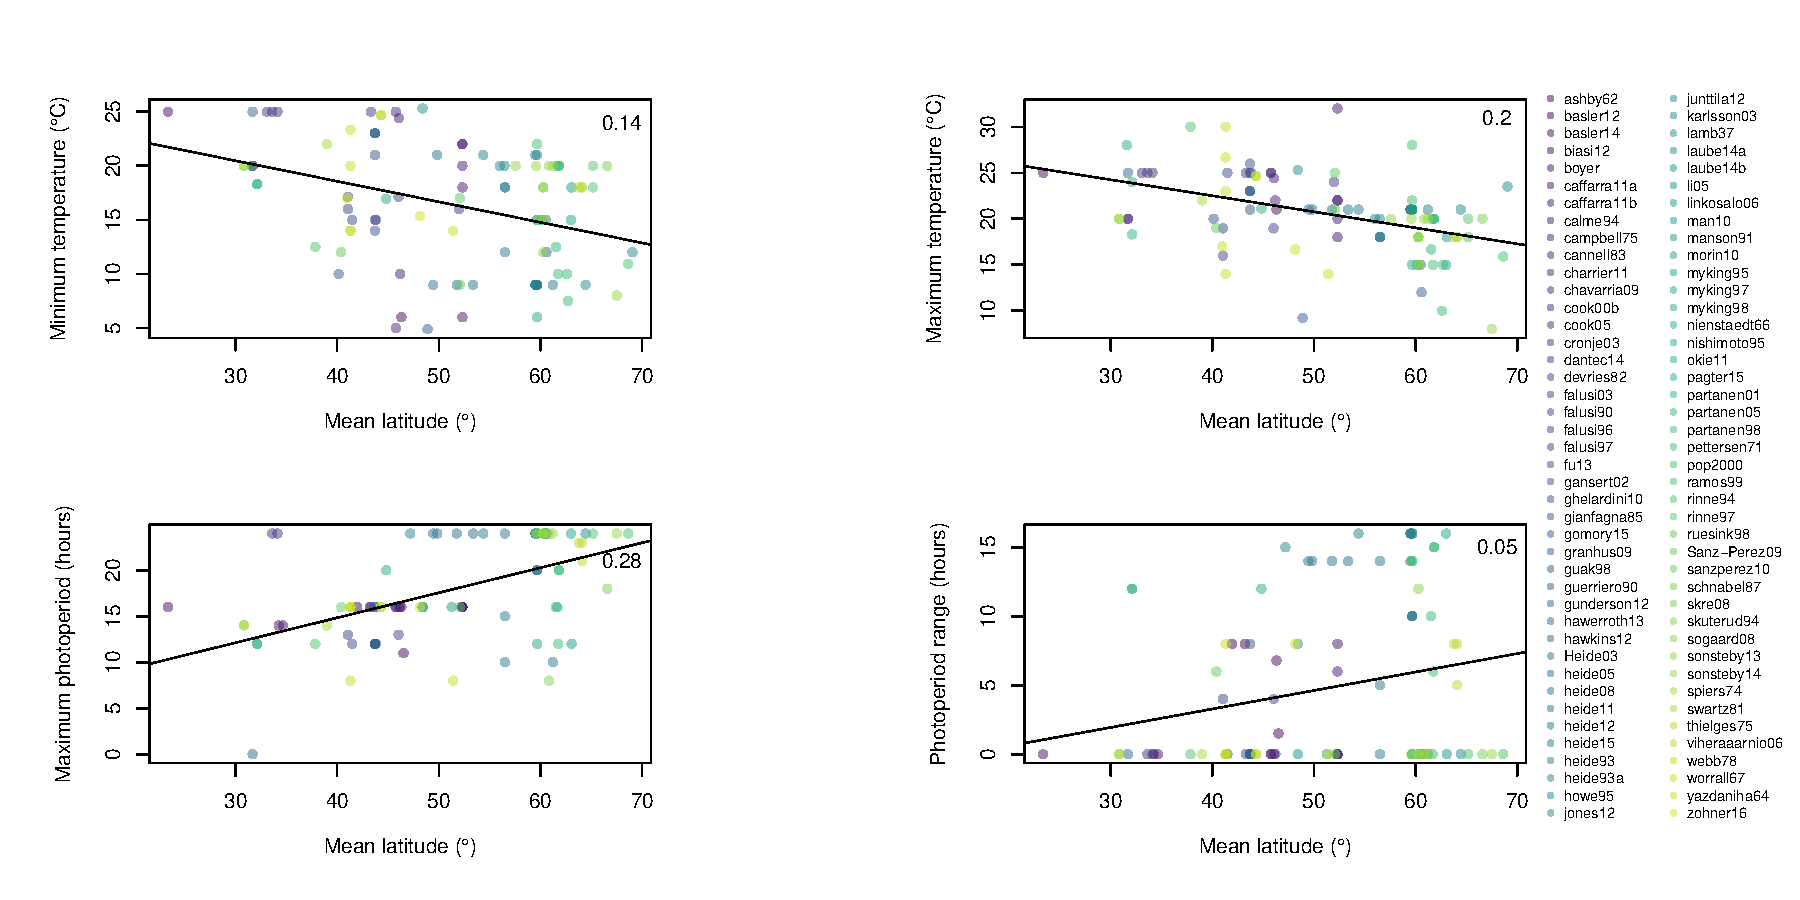
\includegraphics[width=1\textwidth]{..//..//analyses/limitingcues/figures/supplatplots4panel.pdf}
\caption{Experimental treatments correlate with latitude. Here we show the average latitude of a study (averaged over all latitudes from which tissue was taken) versus the minimum (upper left) and maximum (upper right) forcing treatments and the maximum (lower left) photoperiod treatment and range of photoperiod treatments (lower right, range calculated as maximum versus minimum treatments in a study). Colors represent unique datasets (see Table \ref{tab:ref}) and $R^2$ values are given in the upper-right corner of each plot.}
  \label{fig:lat}
\end{figure}
% studydesignplots.R


\end{document}





